\section{Introduction}
%
Since the end of the 20th century, wireless networking is experiencing explosive growth, driven by the popularity of wireless telephony on one hand, and by the development of wireless computer networks on the other hand. Both trends are currently merging into a single attempt: enabling massive wireless Internet access. This phenomenon was inspired by Norman Abramson's pioneer work on packet radio networks \cite{ABRAMSON-70} in the 1970s, and made possible by the authorization of wireless spectrum use for civil telecommunication purposes, in the 1980s\footnote{ISM (Industrial, Scientific, Medical) bands, released in 1985 by US Federal Communications Commission (FCC) for unlicensed use.}. At first, this deregulation encouraged the democratization of wireless telephony, in the 1990s, thanks to the availability of cheaper, more efficient hardware stemming from Cold War military industry efforts. Since 2000, the introduction of new wireless communication standards using the spectrum authorized for civil use has also fueled the development of wireless computer networks and wireless Internet access.
%
\subsection{Managed Wireless Networks}
%
Wireless Internet access is nowadays mostly provided via link layer technologies such as Wifi (IEEE 802.11 infrastructure mode standards \cite{IEEE-802-11}), WiMAX\footnote{Worldwide Interoperability for Microwave Access.} (IEEE 802.16 \cite{IEEE-802-16}), UMTS\footnote{Universal Mobile Telecommunications System.} or LTE\footnote{Long Term Evolution.} (3GPP standards \cite{3GPP}), on user terminals such as smartphones, tablets, laptops, {\em etc}. Such technologies have in common a communication model that is similar to the local wired network model: user terminals (hereafter denominated \glslink{host}{\em hosts}) access the Internet through a dedicated, authoritative infrastructure device (hereafter denominated \glslink{router}{\em router}). In that sense user terminals are competing ``consumers" of the same networking resource, which consists locally in access to the \glslink{router}{router} granting internetwork (Internet) connectivity. \glslink{router}{Routers}, on the other hand, are ``providers" of the networking resource, and collaborate with one another to provide this resource, \emph{i.e.} internetwork connectivity. This similarity enables IPv4 and IPv6 protocol suites to run quite naturally over such wireless access networks, although IP protocols were in fact designed for wired networks at a time when massive use of wireless Internet access was not yet envisioned. \ \\ \ \\
%
The basic mechanisms provided by IEEE 802.11 infrastructure mode, WiMAX, UMTS or LTE thus provide communication capabilities over a single wireless hop, between a user terminal and an infrastructure access point. 
Some extensions of these basic mechanisms provide direct device-to-device communication (as the Wifi ad hoc mode) or even multi-hop wireless communication through relays planned in advance ({\em e.g.} with LTE or WiMAX). However, these wireless networks all have in common their \emph{managed} nature: they depend entirely on an infrastructure planned and deployed in advance, controlled by an operator. This chapter does not focus on such networks.

\subsection{Spontaneous Wireless Networks}
\label{ss:spontaneous}
%
Although so far not as successful as managed wireless networking, an alternative type of wireless networks has also emerged since 2000: \emph{spontaneous wireless networks}. Inspired by the Push-To-Talk concept used in walkie-talkies (portable half-duplex radio transceivers developed during the Second World War), spontaneous wireless networks depart from the traditional distinction between \glslink{router}{routers} and \glslink{host}{hosts}, whereby each user terminal (hereafter, {\em node}) may behave as a \glslink{router}{router} and a \glslink{host}{host} simultaneously. In spontaneous wireless networks, user terminals are thus ``prosumers" ({\em i.e.} both producers and consumers) of networking resources instead of mere consumers. Terminals self-organize to provide multi-hop wireless communications among themselves, with or without help/control from infrastructure devices. Each node may thus simultaneously originate/receive traffic (role of a \glslink{host}{host}), as well as forward traffic on behalf of other terminals (role of a \glslink{router}{router}). \ \\ \ \\ 
%
Popular examples of spontaneous wireless networks include mobile ad hoc networks, wireless mesh networks, wireless sensor or actuator networks, wireless smart meter networks, vehicular networks, opportunistic wireless networks or delay tolerant networks. Spontaneous wireless networks are considered as interesting solutions to extend and offload managed wireless networks hampered by increasingly heavy smartphone data communications \cite{NY-TIMES}. They can also increase the resilience of the network in scenarios where infrastructure is not usable, due to a disaster, to the military situation or to the political situation, for instance \cite{COMMOTION}. In addition, spontaneous wireless networking is an effective way to extend the reach of wireless Internet access, without costly additional infrastructure deployment \cite{OLPC}. \ \\ \ \\ 
%
Popular link layer technologies providing device-to-device communication in spontaneous networks include so far IEEE 802.11 ad hoc mode \cite{IEEE-802-11} and IEEE 802.15.4 \cite{IEEE-802-15.4}. However, in order to provide multi-hop communication in spontaneous wireless networks, additional techniques have to be employed on top of such link layer technologies, and that is the subject of this chapter. The focus is put on the use of standard IP protocols to enable multi-hop wireless communications in spontaneous wireless networks -- in order for these networks to effectively blend in the Internet, where appropriate.%\ \\ \ \\
%
\paragraph{Handling heterogeneity at layer 3} Since the early days of computer networking and the first steps of today's Internet, the diversity of networking technologies has been handled exclusively at the physical and the link layers (layers 1 and 2 OSI). The internetworking layer (layer 3) has been conceived as a ``convergence layer" in which a single protocol (the Internet Protocol, IP) runs unchanged on top of heterogeneous interconnected networks, as it can be observed in Figure \ref{f:conv} \cite{miya}.

\begin{figure}[ht]	% H-must be here or [htb]
\centering
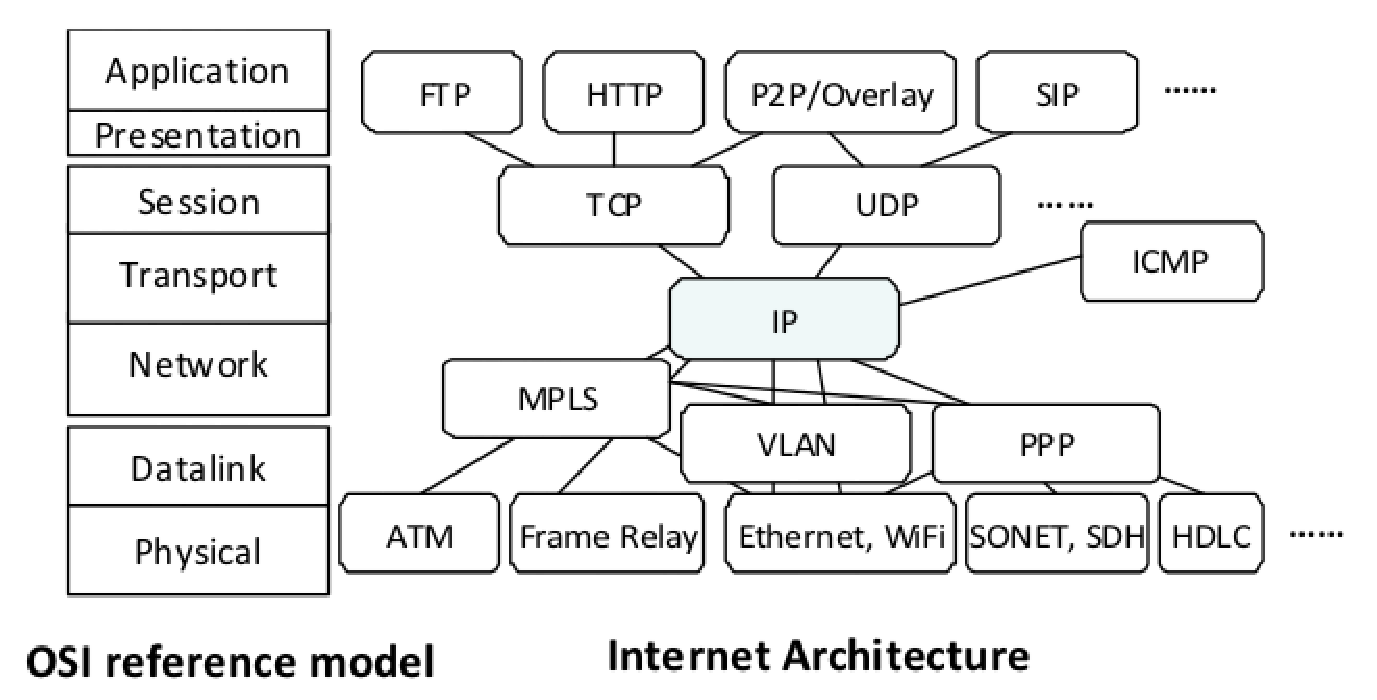
\includegraphics[width=0.7\textwidth]{Figures/protostack-crop.pdf} %	** if .eps or .pdf, don't need extension}
\caption{OSI reference model and IP networking architecture \cite{miya}.}
\label{f:conv}
\end{figure}
%
The development of wireless technology entails however substantial changes in the way that networks are usually represented and conceived. Characteristics of spontaneous wireless networks cannot be handled exclusively at lower layers of communication, as they challenge some of the key assumptions of the IP-based networking architecture. They need thus to be taken into account at layer 3. As more flexible wireless networks are deployed and get increasingly interconnected and integrated with other networks --or in the Internet--, the use of IP over these networks need thus to be adapted or reconsidered. The {\bf first contribution} of the chapter is a review of these considerations, as it elaborates on how the IP-based network architecture is challenged by spontaneous wireless networks.
%
\subsection{Mobile Ad hoc and Low-Power Lossy Networks}
\label{ss:manet_lln}
%
IP protocols are developed, standardized and maintained by the Internet Engineering Task Force (IETF \cite{IETF}). Most of the IETF's protocol design and standardization activities have so far focused on two categories of spontaneous wireless networks: Mobile Ad hoc Networks (MANETs) and Low-Power Lossy Networks (LLNs).

% ({\em e.g.}, a \glslink{router}{router} with multiple \glslink{host}{hosts} and wireless communications devices)--herein simply referred to as `nodes'--

\paragraph{Mobile Ad hoc Networks (MANETs)} According to the IETF's terminology (defined in RFC 2501 \cite{rfc2501}), a MANET consists in a set of ``mobile platforms (..) --herein simply referred to as `nodes'-- (..) which are free to move about arbitrarily. The nodes may be located in or on airplanes, ships, trucks, cars, perhaps even on people or very small devices, and there may be multiple \glslink{host}{hosts} per \glslink{router}{router}. A MANET is an autonomous system of mobile nodes. The system may operate in isolation, or may have gateways to and interface with a fixed network" \cite{rfc2501}. Note that this definition {\em allows} \glslink{router}{router} mobility, but it is {\em not restricted} to mobile networks; the term includes all wireless multi-hop ad hoc networks, regardless of whether they are static or not. 

\paragraph{Low-Power Lossy Networks (LLNs)} According to the IETF's terminology (defined in \cite{draft_lln}), LLNs are ``typically composed of many embedded devices with limited power, memory, and processing resources interconnected by a variety of links, such as IEEE 802.15.4, LowPower WiFi" \cite{draft_lln}. LLNs are thus a more specific case of MANETs (as defined in the previous paragraph), in which \glslink{router}{routers} typically operate with constraints on processing power, memory, and energy (battery power). Their interconnections are characterized by high loss rates, low data rates, and link instability.  LLNs are comprised of anything from a few dozen to thousands of \glslink{router}{routers}.  Supported traffic flows include point-to-point (between devices inside the LLN), point-to-multipoint (from a central control point to a subset of devices inside the LLN), and multipoint-to-point (from devices inside the LLN towards a central control point). Alternative, but similar terminology is employed in {\tt draft-ietf-lwig-terminology} \cite{bormann13}, which defines the terms ``constrained nodes" and ``constrained networks" with various classes of constraints. \\

Concrete examples of MANETs and LLNs include the following three use cases, selected only for illustrative purposes, to hint at the wide heterogeneity of features, requirements and user expectations that one must address in spontaneous wireless networking.

\paragraph{Vehicular Ad hoc Networks (VANETs)} Communication in VANETs is enabled between moving vehicles in urban scenarios or roadways, (possibly) with fixed devices installed in Roadside Units (RSUs) along the road/street. The combination of vehicles and RSUs forms a mobile, highly dynamic ad hoc network. Devices participating in vehicular networks (either inside vehicles or in RSUs) have neither significant energy constraints nor severe computational limitations, but those installed in vehicles are not, in general, cooperative and willing to dedicate resources to others' communication. Research in these networks has typically focused on safety applications, such as distribution along the highway of information about traffic-related events -- \emph{e.g.}, jams or accidents \cite{bc_vanet}. Other purposes could be also considered, such as dissemination of service availability along the highway (gas stations, tolls, accommodation, etc.). As such, a VANET is a category of MANET.

\paragraph{Community Wireless Mesh Networks} These are cooperative, non-commercial networking projects in which users join and contribute to the deployment of the network, in particular by sharing resources and allowing the use of their devices as networking relays. Several initiatives have flourished in the last years, such as Spain's {\em Guifi} \cite{GUIFI}, mostly deployed over the Eastern coast of Spain (Catalonia and Valencia) but also present in many other parts of the country. Other examples include Germany's {\em Freifunk} \cite{FREIFUNK} and Austria's {\em Funkfeuer} \cite{FUNKFEUER}. Some of them cover large geographical areas and contain thousands of nodes\footnote{{\em Guifi.net}, for instance, claims 31865 nodes, 20425 of them being ``operating nodes" (last query to {\tt http://www.guifi.net} on April 10th, 2013).}. These networks are typically static, most of the links are wireless links operating in free (unlicensed) frequency bands. Their topology and capacity evolve dynamically, in an unplanned manner, subject to events such as the ingress and egress of users, the subsequent availability of new links and resources or the upgrade of a particular networking region. These networks enable free communication among their users, but they can also provide access to the Internet if there are gateways available. As such, a community wireless mesh networks is also a category of MANET.

\paragraph{Wireless Sensor Networks (WSNs)} WSNs are collections of sensors intended to measure one or several properties of the environment in which they are deployed. Communication facilities required by such networks need to include, at least, the transmission of collected information from the sensors to a gateway or central server that stores and eventually process it, and the transmission of information (\emph{e.g.}, configuration instructions or measurement schedules) from the server to one or more sensors. There is a broad range of information that may be collected and exchanged through WSNs, some examples including climate studies, bird observation, power monitoring in buildings or tracking of patients' health parameters with body sensors. Properties of a WSN may vary depending on the purposes of the sensor deployment, but there are some usual constraints. Sensors are often battery driven, the lifetime of the sensor is limited by the battery lifetime. Protocols for enabling communication within WSNs must therefore be designed with energy consumption and energy-efficiency in mind. As such, a wireless sensor network is a category of LLN.\\

Despite their heterogeneity, these use cases -- and other applications of spontaneous wireless networks -- have common characteristics, including bandwidth scarcity and need for self-organization. These characteristics both require the use of efficient, highly decentralized routing and flooding mechanisms, able to react quickly to topology changes without overloading the network. This chapter thus focuses more specifically  on IP protocols that enable routing and flooding in MANETs and LLNs. While plenty of protocols have been proposed in the literature, only few have been effectively implemented, standardized and used in real-world deployments. The {\bf second contribution} of the chapter consists in:

\begin{enumerate}[(1)] 
\item an analysis of the main implications of wireless mesh characteristics on the task of flooding and routing typically implemented in upper-layer protocols; and 
\item a description and discussion of the key mechanisms and operation of the main protocols deployed so far and standardized at the IETF for routing in MANETs, in LLNs and in heterogeneous wired/wireless inter-networks.
\end{enumerate}

\subsection{Reader's Guide}

Reader is assumed to be familiar with the main concepts of computer networking and the TCP/IP network reference model, whose terminology is used in this chapter. Interested readers are referred to the book of Tanenbaum {\em et al.} \cite{tanenbaum} for details; the glossary at the end of the chapter displays standard definitions of the basic networking concepts. Basic knowledge of the Internet Protocol (IP) operation, addressing model, routing and Internet architecture is also preferable, but not necessary. These elements are briefly overviewed in section \ref{s:fundamentals}, in order to better highlight the issues that arise with the traditional IP model in spontaneous wireless networks, addressed in section \ref{s:comm_wless}. This section describes the conditions under which wireless communication occurs, and examines their impact on the communication performance and the architecture of spontaneous wireless networks. In particular, the section explains the non-suitability of the conventional IP networking model for spontaneous wireless networks, and discusses an alternative model. \ \\ \ \\ 
%
The rest of the chapter focuses on the mechanisms and protocols that have been designed to handle flooding and routing in spontaneous wireless networks, paying a particular attention to the efforts deployed at the IETF. Section \ref{s:flood_rtg} motivates and presents the mechanisms, and section \ref{s:specific} describes the routing and flooding protocols that have been specifically designed in the IETF to operate on MANETs and LLNs. Section \ref{s:wospf} focuses on the problem of extending legacy Internet routing protocols so that they can efficiently operate on hybrid (wired/wireless) inter-networks. Finally, section \ref{sec:conclusion} concludes the chapter.
